\documentclass[10pt,aspectratio=169]{beamer}
%\setbeameroption{show notes on second screen=right}

%\usetheme{Madrid}


\usetheme[progressbar=frametitle]{metropolis}
\usecolortheme{rose} %beaver, dolphin, crane, 


\setbeamersize{text margin left=4mm, text margin right=4mm}


\usecolortheme{default}
\setbeamertemplate{navigation symbols}{}
\setbeamertemplate{footline}[frame number]
\usepackage[utf8]{inputenc}
\usepackage[T1]{fontenc}

\usepackage{amsmath, amssymb, bm}
\usepackage{booktabs}
\usepackage{graphicx}
\usepackage{ragged2e}
\usepackage{hyperref}
%\hypersetup{colorlinks=true, urlcolor=blue}

\setbeamercolor{item}{fg= orange!80} % Change bullet color
\setbeamercolor{button}{bg=orange, fg=white}

\title[Competing under Information Heterogeneity]{Competing under Information Heterogeneity:\\ Evidence from Auto Insurance}
\author[Cosconati, Fan, Jin, Wu]{Marco Cosconati \and Yi Xin Fan \and Yizhou Jin \and Wu}
\institute{}
\date{\today}

\begin{document}

% 1
\begin{frame}
  \titlepage
\end{frame}



% --- Slide 2: This Paper ---
\begin{frame}{This Paper}

\begin{itemize}
    \item We develop and estimate a novel model of imperfect competition in selection markets:
    \begin{itemize}
        \item Firms have \textbf{heterogeneous information} about consumers.
        \item Differ in cost structure.
        \item Offer differentiated products.
    \end{itemize}
    \medskip % Adds a bit of space between main points
    
    \item We apply our method to study the Italian auto insurance industry:
    \begin{itemize}
        \item \textbf{Substantial differences} in the precision of risk rating and cost structures across firms.
        \item Insurers with more accurate risk rating algorithms \textbf{cream-skim} low-risk consumers, but they tend to have less efficient cost structures.
    \end{itemize}
    \medskip
    
    \item Equalizing information access through a centralized bureau:
    \begin{itemize}
        \item Significantly lowers market prices by increasing competition.
        \item Boosts consumer surplus by 15.7\%, nearly reaching the efficiency benchmark.
        \item Reduces costs by 12 euros per contract through more efficient insurer-insuree matching.
    \end{itemize}
\end{itemize}

\end{frame}

% --- Slide 3: Related Literature ---
\begin{frame}
\frametitle{Related Literature}

\begin{itemize}
    \item The first tractable empirical framework for analyzing imperfect competition when firms have heterogeneous information about consumers.
    \begin{itemize}
        \item Recent empirical studies assume information is symmetrically distributed. \\
        \small{(Cabral et al., 2018; Crawford et al., 2018; Nelson, 2018; Decarolis et al., 2020; Jaffe and Shepard, 2020; Curto et al., 2021; Cuesta and Sepúlveda, 2021; Tebaldi, 2024)}
    \end{itemize}
    \medskip

    \item We extend the classic demand estimation method (Berry, 1994; Berry et al., 1995) to address the common challenge of missing full price menus.
    \begin{itemize}
        \item Prevalent in many empirical analyses \\
        \tiny{(Goldberg, 1996; Cicala, 2015; Crawford et al., 2018; Allen et al., 2019; D'Haultfoeuille et al., 2019; Salz, 2022; Sagl, 2023)}
        \item Wu and Xin (2024) provide more theoretical results and technical details.
    \end{itemize}
    \medskip

    \item On the policy side:
    \begin{itemize}
        \item Antitrust policies and consumer protection with the rise of big data \\
        \tiny{(Lam and Liu, 2020; Jin and Wagman, 2021; Krämer, 2021; Alcobendas et al., 2023; Jeon et al., 2023)}
        \item Financial market regulation \\
        \tiny{(Einav et al., 2013; Chatterjee et al., 2023; Blattner et al., 2022; Nelson, 2025; Blattner and Nelson, 2021; Liberman et al., 2018; Hertzberg et al., 2011)}
    \end{itemize}
\end{itemize}

\end{frame}

% --- Slide 4
\begin{frame}
\frametitle{Data}
    \begin{itemize}
        \item A representative sample of matched insurer-insuree panel in Rome (2013-2021).
        \begin{itemize}
            \item Customers with tenure=0, top 10 firms + fringe firms (Firm 11).
        \end{itemize}
        
        \medskip
        \item We observe: \textbf{Summary Statistics}
        \begin{itemize}
            \item Risk factors: age, bonus-malus, residence, vehicle features, driving records, etc.
            \item Premium, coverage, and contract clauses.
            \item Frequency and severity of claims at each contractual year.
            \item \textbf{Substantial variation in premiums and claim payouts across firms.} \textbf{Details}
        \end{itemize}
        
        \medskip
        \item We don't observe:
        \begin{itemize}
            \item Full price menu (only transaction prices).
            \item Full set of pricing variables (factors in the data explain 50\% of price variation). \textbf{Details}
            \item Insurers incorporate \textbf{different} variables into their actuarial models. \textbf{Survey}
        \end{itemize}
    \end{itemize}
\end{frame}

% --- Slide 5
\begin{frame}{Do Insurers Differ in Risk Assessment Precision?}
    \begin{columns}[T] % The [T] option aligns the columns at the top
        
        % Left Column (for the graph)
        \begin{column}{0.5\textwidth}
            % Note: You need to have the image file in the same folder 
            % or provide the correct path. I'm using a placeholder.
            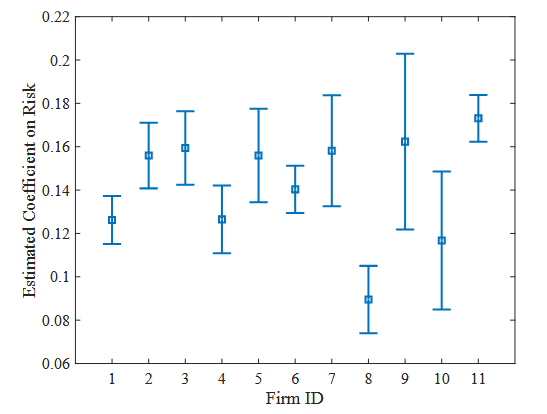
\includegraphics[width=\linewidth]{Figures/Fig2.png} 
        \end{column}
        
        % Right Column (for the text)
        \begin{column}{0.5\textwidth}
            \begin{itemize}
                \item Regressing premiums on \textbf{ex-post} realized claims. \textbf{Details}
                
                \medskip
                \item Certain firms' premiums are \textbf{more responsive to}, or more \textbf{accurately reflect}, estimated ex-post risk.
                
                \medskip
                $\implies$ These firms are potentially \textbf{more informed} and better at assessing consumer risk.
            \end{itemize}
        \end{column}
    \end{columns}
\end{frame}

% --- Slide 6: Model ---
\begin{frame}{Model}
    \begin{itemize}
        \item A static model of price competition among $J$ insurers, indexed by $j=1, 2, \dots, J$.
        
        \medskip
        \item Each firm offers a standardized insurance product.
        
        \medskip
        \item Consumer's risk type $\theta$: expected claim payouts.
        \begin{itemize}
            \item Ex-ante not observed by the firms;
            \item Population distribution $f_0(\theta)$ is common knowledge.
        \end{itemize}
    \end{itemize}
\end{frame}

% --- Slide 7: Signal Structure ---
\begin{frame}{Signal Structure}
    \begin{itemize}
        \item For a consumer of type $\theta$, firm $j$ draws a signal $\hat{\theta}_j \sim N(\theta, \sigma_j^2)$, with density $\phi(\hat{\theta}_j; \theta, \sigma_j)$.
        
        \medskip
        \item $1/\sigma_j$ measures firm $j$'s information precision.
        
        \medskip
        \item Signals are \textbf{private} and independent \textbf{conditional on} $\theta$.
        
        \medskip
        \item Related to common value auctions: signals are noisy estimates of the true but unknown common value, i.e., the cost to insure the consumer.
    \end{itemize}
\end{frame}


% --- Slide 8: Risk Rating ---
\begin{frame}{Risk Rating}
    \begin{itemize}
        \item Firms infer the risk of the consumer upon observing the signal.
    \end{itemize}
    
    \vspace{1cm} % Add some vertical space
    
    \centering
    $E(\theta | \hat{\theta}_j, D=j) = \int_{\theta} \theta f(\theta | \hat{\theta}_j, D=j) d\theta = \frac{\int_{\theta} \theta \overbrace{\Pr(D=j | \hat{\theta}_j, \theta)}^{\text{Selection Prob.}} \phi(\hat{\theta}_j; \theta, \sigma_j) f_0(\theta) d\theta}{\int_{\theta} \Pr(D=j | \hat{\theta}_j, \theta) \phi(\hat{\theta}_j; \theta, \sigma_j) f_0(\theta) d\theta}$
    
    \vspace{1cm}
    
    \begin{itemize}
        \item $E(\theta | \hat{\theta}_j, D=j)$ is an \textbf{equilibrium} object.
        
        \item $f$ is posterior dist of $\theta$ conditional on the signal and the consumer being \textbf{selected} into the firm.
        
        \item Selection probability depends on \textbf{all firms'} pricing strategies through consumers' demand.
    \end{itemize}
\end{frame}

% --- Slide 9: Pricing Strategy ---
\begin{frame}{Pricing Strategy}
    \begin{itemize}
        \item Firm $j$ sets the price based on the risk evaluation:
    \end{itemize}

    \[
    p_j(\hat{\theta}_j) = \alpha_j + \beta_j \underbrace{E(\theta | \hat{\theta}_j, D=j)}_{\text{risk rating}}.
    \]

    \begin{itemize}
        \item $\alpha_j$ and $\beta_j$ are pricing coefficients \textbf{optimally} chosen by the firm.
        
        \item $\alpha_j$ relates to the baseline markup; $\beta_j$ relates to the elasticity of price wrt risk.
    \end{itemize}
\end{frame}

% --- Slide 10: Demand ---
\begin{frame}{Demand}
    \begin{itemize}
        \item Firms offer homogeneous insurance plans, but may have \textbf{unobserved} (by the econometrician) product attributes $\xi_j$, such as service quality or brand loyalty.
        
        \medskip
        \item The utility derived by a consumer $i$ for a product from firm $j$:
        \[ U_{ij} = -\gamma_i p_j(\hat{\theta}_j) + \xi_j + \varepsilon_{ij}. \]
        $\varepsilon_{ij}$'s are iid utility shocks from type I extreme value dist.
        
        \medskip
        \item The probability that a consumer chooses firm $j$ given $\hat{\theta} = (\hat{\theta}_1, \hat{\theta}_2, \dots, \hat{\theta}_J)$:
        \[ \Pr(D=j|\hat{\theta}) = \frac{\exp(-\gamma_i p_j(\hat{\theta}_j) + \xi_j)}{\sum_{j'=1}^{J} \exp(-\gamma_i p_{j'}(\hat{\theta}_{j'}) + \xi_{j'})}. \]
        
        \medskip
        \item Could also allow demand parameters $(\gamma, \xi)$ to vary with $\theta$.
    \end{itemize}
\end{frame}

% --- Slide 11: Profit Maximization ---
\begin{frame}{Profit Maximization}
    \begin{itemize}
        \item Firms simultaneously choose pricing coefficients $(\alpha_j, \beta_j)$ to maximize expected profits, given common knowledge of all firms' primitives (e.g., signal distributions, costs) and $f_0(\theta)$.
        
        \medskip
        \item Firm $j$'s profit $\pi_j(\alpha, \beta)$
        
        \[
        \int_{\hat{\theta}} \int_{\theta} \underbrace{(p_j(\hat{\theta}_j) + c_j - k_j\theta)}_{\text{net profit}} \underbrace{\Pr(D=j|\hat{\theta})}_{\text{choice prob.}} \underbrace{\left(\prod_{j'=1}^{J} \phi(\hat{\theta}_{j'}; \theta, \sigma_{j'}) \right)}_{\text{signal dist.}} \underbrace{f_0(\theta)}_{\text{type dist.}} d\theta d\hat{\theta}.
        \]
        
        \medskip
        \item $c_j$: ``net benefits'' of contracting with a customer irrespective of the risk.
        
        \item $k_j$: efficiency at processing claims.
    \end{itemize}
\end{frame}

\section{Estimation}
 
% --- Slide 12: Estimation ---
\begin{frame}{Estimation}
    \begin{itemize}
        \item \textbf{Joint Distribution of Premium and Risk Type:}
        \begin{itemize}
            \item Using a panel of claim records.
        \end{itemize}
        
        \medskip
        \item \textbf{Demand:}
        \begin{itemize}
            \item Market shares $\implies$ unobserved product attributes.
            \item Consumer sorting patterns $\implies$ price sensitivity.
        \end{itemize}
        
        \medskip
        \item \textbf{Supply:}
        \begin{itemize}
            \item Joint distribution of premium and risk within firm $\implies$ pricing coefficients and signal dist.
            \item First-order conditions $\implies$ cost parameters.
        \end{itemize}
    \end{itemize}
\end{frame}

% --- Slide 13: Demand ---
\begin{frame}{Demand}
    \begin{itemize}
        \item Key challenge: observe only transaction prices, not offered prices.
        \begin{itemize}
            \item Auction: observe only winning bids, not submitted bids.
            \item Roy models: observe only accepted wages, not potential wages.
        \end{itemize}
        
        \medskip
        \item The offered and accepted price distributions are linked through the demand system.
        
        \medskip
        \item We propose a novel fixed-point approach that jointly estimates choice probabilities, offered price distributions, and demand parameters.
    \end{itemize}
\end{frame}

% --- Slide 14: Estimation ---
\begin{frame}{Estimation}
    \begin{itemize}
        \item Wu and Xin (2024) construct an operator whose fixed point is the offered price distributions and show that it is a functional contraction.
        
        \medskip
        \item $\xi$: matched to aggregate market shares; $\gamma$: identified from sorting patterns.
        
        \medskip
        \item Possible to allow preference to vary with risk (need parametric assumptions).
        
        \medskip
        \item Key insight for supply-side estimation: offered price \textbf{monotonically increases} with signal (analogy to auction models: bid is a monotone increasing function of valuation).
        
        \medskip
        \item Cost parameters are identified from firms' first-order conditions.
    \end{itemize}
\end{frame}

% --- Slide 15: Demand-Side Results ---
\begin{frame}{Demand-Side Results}
    \begin{columns}[T]
        % Left Column (Table)

        \begin{column}{0.3\textwidth}
          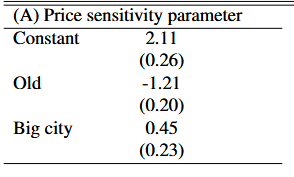
\includegraphics[width=1.2\linewidth]{Figures/Tab2A.png} 
            %\begin{tabular}{lcc}
            %\toprule
            %\textbf{Price Sensitivity} & \textbf{Estimates} & \textbf{Std. Err.} \\
            %\midrule
            %Constant & 2.11 & (0.26) \\
            %Old & -1.21 & (0.20) \\
            %Big city & 0.45 & (0.23) \\
            %\bottomrule
            %\end{tabular}
        \end{column}
        
        % Right Column (Text)
        \begin{column}{0.5\textwidth}
            \begin{itemize}
                \item Senior consumers tend to be less price sensitive.
                \medskip
                \item We allow preferences for unobserved product attributes to vary with risk type, geography, and time.
                \medskip
                \item $\xi$'s are generally similar across low- and high-risk groups.
            \end{itemize}
        \end{column}
    \end{columns}
\end{frame}


% --- Slide 16: Supply-Side Results ---
\begin{frame}
\frametitle{Supply-Side Results}
    \begin{itemize}
        \item Huge heterogeneity along \textbf{all} dimensions.
    \end{itemize}
     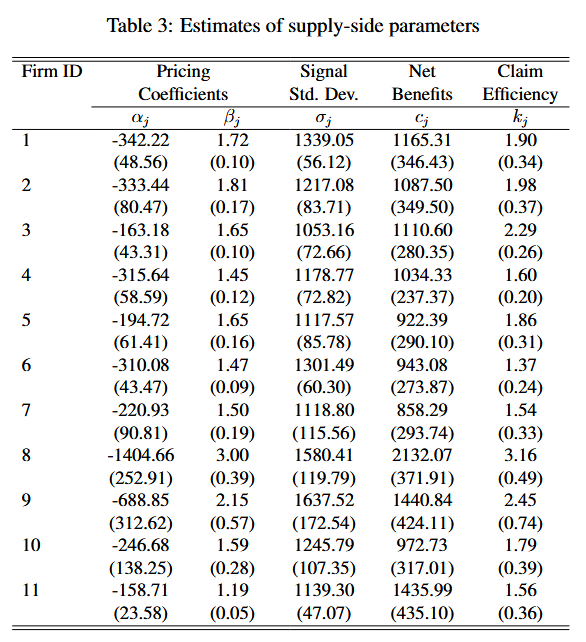
\includegraphics[width=.5\linewidth]{Figures/Tab3.png} 
\end{frame}

\begin{frame}
\frametitle{Supply-Side Results}
    \begin{itemize}
        \item Huge heterogeneity along \textbf{all} dimensions.
    \end{itemize}
     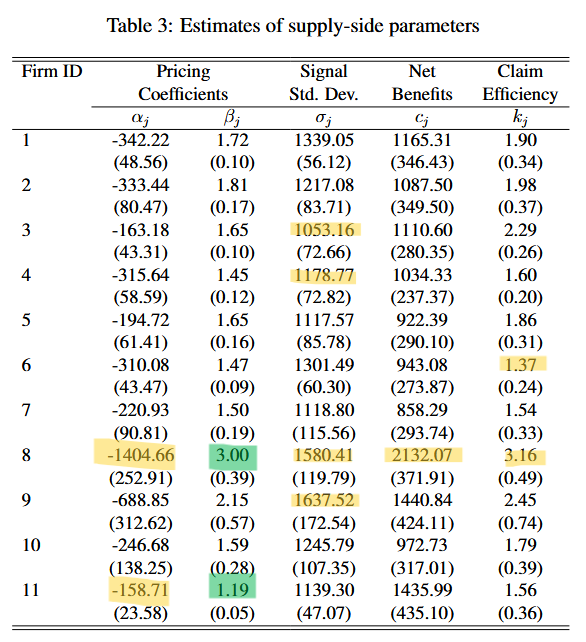
\includegraphics[width=.5\linewidth]{Figures/Tab3_hihglighted.png} 
\end{frame}


% --- Slide 17: Correlations ---
\begin{frame}
\frametitle{Correlations}
    \begin{itemize}
        \item Comparative advantages along different dimensions:
        \begin{itemize}
            \item Firms suffering lower information precision tend to have lower marginal costs.
            \item Firms with higher marginal costs tend to be more efficient at processing claims.
        \end{itemize}
    \end{itemize}
         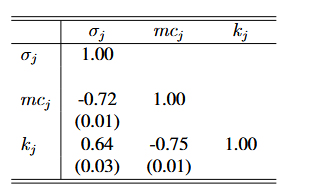
\includegraphics[width=.38\linewidth]{Figures/Tab4.png} 
\end{frame}


\begin{frame}
\frametitle{Correlations}
    \begin{itemize}
        \item Comparative advantages along different dimensions:
        \begin{itemize}
            \item Firms suffering lower information precision tend to have lower marginal costs.
            \item Firms with higher marginal costs tend to be more efficient at processing claims.
        \end{itemize}
    \end{itemize}
         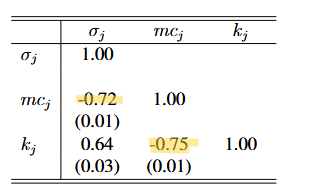
\includegraphics[width=.38\linewidth]{Figures/Tab4_highlighted.png} 
\end{frame}

% --- Slide 18: --- Who goes where?  ---
\begin{frame}
\frametitle{Who Goes Where?}
    \centering
    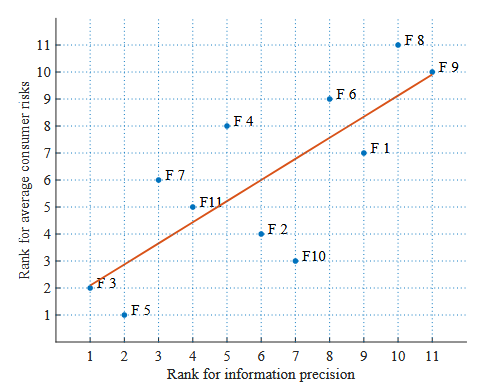
\includegraphics[width=0.6\textwidth]{Figures/Fig4.png} 
\end{frame}

% --- Slide 19: --- Counterfactuals ---
\begin{frame}
\frametitle{Counterfactuals}
    \begin{itemize}
        \item \textbf{Main policy:} establishing a centralized bureau that collects signals from all firms and aggregates them based on information precision. The posterior estimate of each consumer's risk given \textbf{all signals} $E(\theta|\hat{\theta})$ is made public.
        
        \medskip
        \item An \textbf{efficiency benchmark:} the true risk type of each consumer is observed by all firms $\implies$ information asymmetry is completely eliminated.
        
        \medskip
        \item A \textbf{privacy benchmark:} firms are required to limit their use of consumer data, $\sigma$ is set to be the largest currently observed in the market $\implies$ reduce overall information availability.
    \end{itemize}
\end{frame}

% --- Slide 20 --- Sorting Patterns
\begin{frame}{Sorting Patterns}
    \begin{columns}[T]
        % Left Column (Graph)
        \begin{column}{0.6\textwidth}
            \centering
            % Replace 'sorting_patterns.png' with your actual image file.
            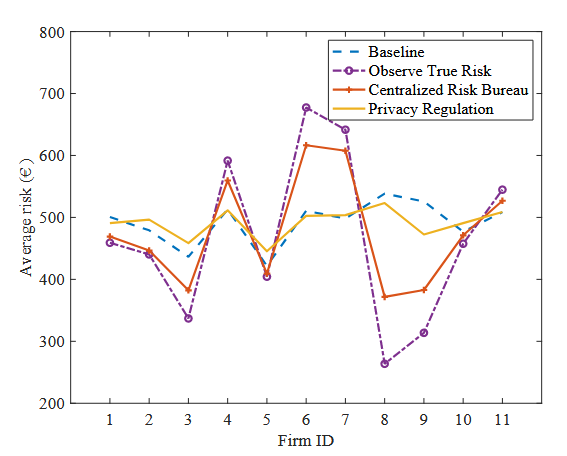
\includegraphics[width=.9\linewidth]{Figures/Fig6.png}
        \end{column}
        
        % Right Column (Text)
        \begin{column}{0.4\textwidth}
            \begin{itemize}
                \item Sorting under full information or centralized risk bureau is driven by specialization based on cost advantages.
                
                \medskip
                $\implies$ Improve market efficiency (reduce the avg cost by 3.7\%).
                
                \medskip
                \item Sorting nearly disappears under privacy regulation.
            \end{itemize}
        \end{column}
    \end{columns}
\end{frame}

\begin{frame}
\frametitle{Conclusions}
    \begin{itemize}
        \item Our paper develops a novel empirical framework for studying competition under information heterogeneity.
        
        \medskip
        \item We focus on Italian auto insurance industry: substantial differences in the precision of risk rating across firms; however, firms with lower information precision tend to have lower costs.
        
        \medskip
        \item We evaluate the \textbf{equilibrium effects} of a public information policy where insurers' risk estimates are aggregated and made public through a centralized bureau:
        \begin{itemize}
            \item a significant price reduction due to increased competition.
            \item boosts consumer surplus by 15.7\%, nearly matching the efficiency benchmark.
            \item improves the matching efficiency between insurers and insurees.
        \end{itemize}
    \end{itemize}
\end{frame}


\end{document}
